\section{Wstęp teoretyczny}

\subsection{Historia sztucznej inteligencji.}
\begin{par}
Na początku lat 40 matematycy i inżynierowie z ośrodków badawczych zaczęli zastanawiać się nad możliwością stworzenia sztucznego mózgu.
Pierwsze formalne centrum badawcze pracujące nad zagadnieniem sztucznej inteligencji zostało powołane do życia w 1956 roku w Dartmouth College, 16 lat po wynalezieniu pierwszego programowalnego komputera.
Początkowo nazywane przedsięwzięciem stworzenia pierwszego ``Elektronicznego mózgu'' zostało poważnie potraktowane przez ówczesnych naukowców, i tworzyło dobre perspektywy dla ekonomistów i bankierów.
Wielu badaczy zapowiedziało stworzenie maszyn dorównujących inteligencją ludziom w niespełna kilka dekad.
Specjalnie na ten cel rząd amerykański oraz brytyjski przeznaczyły budżet rzędu milionów dolarów.
\end{par}
\begin{par}
Pierwsze prace nad sztuczną inteligencją skupiały się na odwzorowaniu realnej pracy ludzkiego mózgu - sieci neuronów.
Naukowcy tacy jak Norbert Wiener, Claude Shannon oraz Alan Turing opracowali pierwsze pomysły stworzenia elektronicznego mózgu.
Powstało pojęcie sieci neuronowych, mocno później rozwijane m.in. przez Marvina Minskiego w jego pracach przez następne 50 lat.
Pierwsze programy skupiające się na sztucznej inteligencji w grach powstały na początku lat 50. Christopher Strachey był autorem pierwszego programu grającego w Warcaby.
Pierwszy program szachowy został napisany przez Dietricha Prinza.
W tym samym okresie Alan Turing opublikował pierwsze prace dotyczące możliwości utworzenia maszyny dysponującej ludzką inteligencją.
Zdefiniował test pozwalający to zmierzyć, nazywany potem Testem Turinga.
\end{par}
\begin{par}
W końcu po wielu latach stało się oczywiste iż symulacja nawet najprostszych mechanizmów myślowych jest niezwykle trudna w realizacji, a nawet najszybsze ówczesne komputery nie były w stanie wygrać z człowiekiem w partii szachów. 
Ostatecznie dziedzinie sztucznej inteligencji odebrano nieco wiarygodności, a wcześniej zapowiadane maszyny przerastające inteligencją ludzi, trafiły z powrotem na półki science-fiction. W roku 1973, znaczna część funduszy przeznaczonych na rozwój sztucznej inteligencji została wstrzymana przez amerykański i brytyjski rząd.
Niemniej prace nad sztuczną inteligencją trwają do dziś, aczkolwiek są bardziej uszczegółowione w naturze problemów których dotyczą.
\end{par}


\subsection{Sztuczna w dzisiejszych zastosowaniach.}
\begin{par}
Oprócz realizacji zadań w dziedzinie kategoryzacji danych, oraz rozpoznawaniu mowy lub obrazu, spora część badań skupia się na realizacji systemów podejmujących decyzje w ściśle określonym środowisku gry.
Pozornie służą one jedynie dostarczaniu rozrywki w szeroko popularnych grach komputerowych, szybko można się przekonać iż wiele takich projektów jest później podstawą do stworzenia bardziej praktycznych systemów. Zmieniając jedynie definicję środowiska okazuje się iż można te same strategie zastosować np. w grze na giełdzie.
Pojedynek Garriego Kasparowa z programem szachowym Deep Blue przeszedł już na stałe do historii jako pierwsze starcie człowieka z maszyną w dziedzinie intelektu. 
Innym, dość nowym przykładem może być klaster komputerów Watson, który przez kilka tygodni konkurował z czołówką graczy teleturnieju Jeopardy, popularnym w USA od 1964 roku.
Obydwa projekty pokonały swoich ludzkich przeciwników, podnosząc tym samym nieco nadszarpnięty wizerunek sztucznej inteligencji.
Wiele współczesnych zastosowań sztucznej inteligencji zyskało dużą popularność dzięki globalnej sieci internet.
Prym wiedzie tutaj firma Google, początkowo znana jedynie jako twórca najpopularniejszej i najdokładniejszej wyszukiwarki, rozbudowuje bazę swoich aplikacji o translatory,
aplikacje do nawigacji map, czy program graficzny Picasa, potrafiący np. zidentyfikować na zdjęciu ludzką twarz.
Większość wyszukiwarek internetowych wykorzystuje różnego rodzaju systemu wspomagające w wyszukiwaniu informacji na temat konkretnej frazy.
Aktywna lista podpowiedzi wyświetlająca się po wpisaniu początku popularnej frazy stała się wręcz standardem w projektowaniu wyszukiwarki.
Wyszukiwarka coraz częściej poprawia błędy ortograficzne lub niepoprawnie przeliterowane wyrazy związane np. z bliskim sąsiedztwem liter na klawiaturze.
Innym ciekawym zastosowaniem jest tłumaczenie tekstu z dowolnego języka na inny.
Nie działa to na zasadzie bazy danych przechowującej odpowiedniki słów w każdym z języków, lecz wykorzystuje metodę ``uczenia się'' całych wyrażeń bądź zwrotów które są równorzędne w obu językach, 
dzięki czemu zyskujemy dość precyzyjne tłumaczenie nawet jeśli chodzi o nazwy własne, akronimy, odmianę oraz składnię, np.: Przy tłumaczeniu z angielskiego na polski frazy ``United States of America'' uzyskujemy ``Stany Zjednoczone'', natomiast ``in UK'' tłumaczone na język polski poprawnie daje zwrot ``w Wielkiej Brytanii''.
W pierwszym przykładzie naiwna metoda nie ominęłaby słowa ``America'' oraz prawdopodobnie nie zachowałaby szyku słów. Wynikiem mogłoby być wówczas ``Zjednoczone Stany Ameryki''.
Inne ciekawe zastosowaniem może być aplikacja Wolfram Alpha stworzona przez Stephena Wolframa.
Podobnie jak wyszukiwarka Google, opiera ona swoje wyniki na frazach wpisywanych do okna wyszukiwarki przez użytkownika, jednak jest ona skupiona głównie na przetwarzaniu danych matematycznych.
Potrafi interpretować wzory wpisane przez użytkownika, wyświetlić wykres w przestrzeni oraz dostarczyć wielu dodatkowych informacji np. znaleźć pierwiastki rzeczywiste.
O ile sztuczna inteligencja w świetle dzisiejszego dostępu ogromu danych do przetwarzania stwarza duży potencjał na tworzenie skomplikowanych systemów przetwarzających wciąż spotykamy
się z jej rosnącym zastosowaniem w grach.
Historia informatyki od jej wczesnych początków związana była z grami komputerowymi. 
W roku 1952 Alexander Shafto Douglas opisał temat komunikacji człowiek-komputer w swojej pracy doktoranckiej, oraz stworzył program grający w popularne ``Kółko i Krzyżyk''.
Do dziś uznawany jest on za pierwszą graficzną grę komputerową.
\end{par}

\subsection{Podstawy algorytmów w grach.}
\begin{par}
Jednym z podstawowych przykładów zastosowania sztucznej inteligencji w grach komputerowych są gry logiczne. 
Podstawowym algorytmem stosowanym w projektowaniu sztucznej inteligencji jest algorytm minmax.
Najprostszym przykładem jest gra ``Kółko i krzyżyk'' gdzie przeszukiwane jest tzw. drzewo gry, kolejno sprawdzające wszystkie możliwe stany gry. 
W dowolnym momencie gry możemy przeanalizować wszystkie możliwe posunięcia każdego z graczy, i dążyć do sytuacji gdzie mamy gwarantowany sukces.
Gra może zakończyć się remisem, zwycięstwem gracza A, bądź zwycięstwem gracza B.
Optymalizując decyzję gracza A, musimy kolejno sprawdzać możliwe posunięcia na planszy i reakcje gracza B. 
Dla każdego z możliwych ruchów nich możemy wówczas przeanalizować optymalną strategię dla gracza B (ponieważ zakładamy że do takiej będzie on dążył) i starać się znaleźć 
najlepszą ścieżkę która prowadzi do zwycięstwa gracza A, bądź remisu.
Łatwo zauważyć iż algorytm taki ma ogromną złożoność dla rozbudowanych drzew, i jedynie dla małych gier takich jak kółko i krzyżyk daje wynik w realnym czasie.
Bez optymalizacji, oraz brania pod uwagę symetrii planszy, daje to drzewo wywołań składające się 9! węzłów (łącznie z liśćmi). 
Oczywiście algorytm można zoptymalizować chociażby poprzez programowanie dynamiczne, lecz dla gier bardziej złożonych nie będziemy w stanie przeanalizować wszystkich możliwych sytuacji w grze w realnym czasie.
Przez lata szachy były jedną z gier niemożliwych do rozwiązania za pomocą powyższego podejścia.
Nawet dziś najlepsze programy szachowe nie grają idealnie - nie analizują wszystkich możliwych ruchów a jedynie kilkadziesiąt ruchów w przód.
Przy zastosowaniu optymalizacji oraz bazy danych zawierającej wiele strategii szachowych, współczesne programy szachowe wygrywają z najlepszymi graczami.
Nieco inna sytuacja jest w grze GO, gdzie plansza rozmiaru 19x19 stanowi duże wyzwanie nawet dla współczesnych superkomputerów. 
Do dziś nie stworzono programu który wygrywałby z profesjonalnymi zawodnikami GO.
Jak widać na Rys. \ref{fig:xo_tree}, pierwsze 2 poziomy drzewa gry Kółko i Krzyżyk nie są zbyt skomplikowane jeśli weźmiemy pod uwagę symetrię.
Początkowo złożoność drzewa rośnie wykładniczo, jednak możliwości na planszy kończą się zanim zaczyna to być problemem.
Inaczej wyglądałby przypadek drzewa gry GO (plansza rozmiaru 13x13), gdzie pierwszy ruch można wykonać na 28 unikalnych sposobów: Rys. \ref{fig:go_tree} przedstawia przykładowe pierwsze 28 węzłów drzewa gry GO (13x13) biorąc pod uwagę symetrię planszy.
Sprawa komplikuje się gdy rozpatrujemy większe plansze.
Dla plansz o wymiarach 19x19 - standardowym rozmiarze obowiązującym na wszystkich turniejach gry GO - pierwszy ruch można wykonać na 55 sposobów (analogicznie do Rys.\ref{fig:go_tree}). Plansza GO ma 4 osie symetrii, może się wówczas okazać że odpowiedź przeciwnika będzie na tyle ``niesymetryczna'', że już na drugim
poziomie drzewa musimy rozpatrzyć wszystkie możliwe pola na planszy, czyli 359 (19x19 - 2).

\begin{figure}[!h]
	\centering
	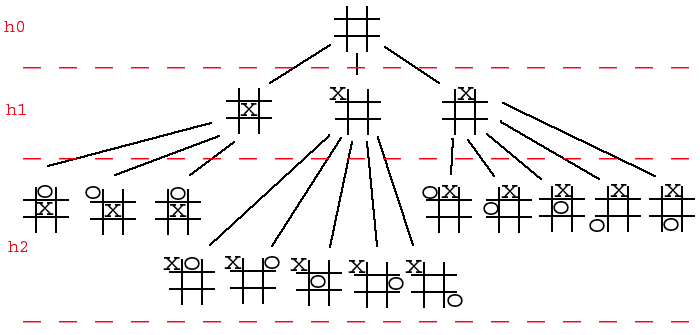
\includegraphics[width=5in]{obrazki/chess_tree.png}
	\caption{Schemat drzewa gry Kółko i Krzyżyk.}
	\label{fig:xo_tree}
\end{figure}

\begin{figure}[!h]
	\centering
	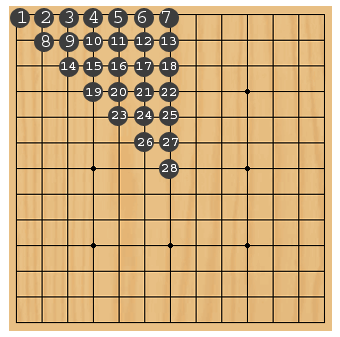
\includegraphics[width=5in]{obrazki/go_tree.png}
	\caption{Przykład pierwszych możliwych unikalnych ruchów w grze GO.}
	\label{fig:go_tree}
\end{figure}

\end{par}
\begin{par}
Jeśli chcemy wprowadzić podział gier przydatny przy projektowaniu systemu pierwszym czynnikiem będzie typ rozgrywki ze względu na czas.
Większość gier można podzielić wówczas w następujący sposób:
\begin{itemize}
	\item Gry turowe - Gracze naprzemiennie wykonują ruchy, przy czym czas na podjęcie decyzji jest relatywnie duży - od 1 sekundy nawet do 1-2 minut.
Wiele nieskomplikowanych gier turowych zostało już dawno rozwiązanych przez algorytmy typu minmax, do tego stopnia, że systemy grają w nie już niemal bezbłędnie. 
W wielu przypadkach przestrzeń rozwiązań jest jednak wciąż zbyt duża aby zrealizować to algorytmem dokładnym - przykładem może być wyżej wspomniana gra GO.
	\item Gry czasu rzeczywistego - Gra toczy się w dynamicznym środowisku gry, często z wieloma obiektami i graczami na raz. Często czas na podjęcie optymalnej decyzji przez algorytm jest mocno ograniczony - często należy podejmować odpowiednie decyzje nawet do 30 razy w ciągu sekundy. Oprócz tego próba dyskretyzacji środowiska i znalezienia dokładnego rozwiązania z przestrzeni stanów gry jest w praktyce niewykonalne. Przykładem mogą być tutaj różnego rodzaju dwu lub trójwymiarowe gry akcji, które często posiadają złożone środowiska gry, wiele dynamicznych obiektów oraz graczy uczestniczących w rozgrywce poprzez przez sieć komputerową. Przy projektowaniu sztucznej inteligencji w takim środowisku w tej chwili możemy liczyć jedynie na wyniki przybliżone.
\end{itemize}
Sztuczna inteligencja w grach może dotyczyć różnych aspektów gry. 
W grach logicznych (turowych) głównym, i jedynym problemem jest podjęcie najlepszej decyzji dla aktualnego stanu gry, prowadzącej do zwycięstwa. 
W większości gier logicznych sztuczna inteligencja ma za zadanie symulację godnego przeciwnika dla człowieka.
Często jednak te same algorytmy mogą służyć do celów edukacyjnych bądź do podpowiedzi - ten sam system grający w szachy może grać przeciwko nam, jak i podpowiadać nam ruchy na podstawie naszej pozycji na planszy.
W grach zręcznościowych oraz akcji (gry czasu rzeczywistego) występuje często inny rodzaj sztucznej inteligencji.
Ponieważ przestrzeń rozwiązań jest bardzo duża, często podjęcie decyzji może być wspomagane przez algorytm przybliżony, bądź oparty na algorytmach genetycznych.
Algorytm minmax w większości przypadków zawodzi, bądź jego czas działania jest zbyt wolny do zastosowania w dynamicznym środowisku gry.
Korzystając z algorytmów ``jedynie'' optymalizujących rozgrywkę tracimy możliwość rozegrania idealnej partii gry, jednak często wystarcza to dla osiągnięcia celu końcowego jakim jest
stworzenie godnego przeciwnika.
\end{par}

\subsection{Podstawy algorytmów genetycznych.}
\begin{par}
Często wykorzystywanym sposobem rozwiązania złożonego problemu algorytmicznego są algorytmy genetyczne.
Opierają się one na zasadach ewolucji odkrytych przez Charlesa Darwina, i wzorują się na faktycznych rozwiązaniach doboru naturalnego występujących w przyrodzie.
Algorytm ewolucyjny opiera się na wprowadzeniu losowego czynnika do całej procedury, i tym też różni się od klasycznego algorytmu, iż jest niedeterministyczny. 
Ogólny przebieg algorytmu genetycznego może wyglądać następująco:
\begin{enumerate}
\item Wygenerowanie początkowej populacji osobników (rozwiązań) w sposób losowy.
\item Przeliczenie funkcji przystosowania dla każdego z osobników.
\item Uporządkowanie populacji malejąco względem wyniku funkcji przystosowania.
\item Wybranie populacji rodzicielskiej zgodnie z przyjętą metodą selekcji.
\item Krzyżowanie osobników z populacji rodzicielskiej i otrzymanie nowej populacji - nowe potomstwo posiada cechy rodziców którzy w poprzedniej populacji byli najlepiej przystosowani do rozwiązania danego problemu.
\item Mutacja części potomstwa - wprowadzenie czynnika losowego poprzez zmianę niektórych fragmentów chromosomu w sposób losowy.
\item Jeśli warunek końcowy nie został osiągnięty powrót do kroku 2, w przeciwnym wypadku koniec algorytmu.
\end{enumerate}
Wynikiem takiego algorytmu jest nie jedno rozwiązanie problemu, a cała ich populacja.
W większości algorytmów genetycznych można wydzielić kilka koniecznych do zaprojektowania klas bądź procedur.
\begin{enumerate}
\item Chromosom oraz Populacja
	\begin{par}
		Pierwszym krokiem jest zdefiniowanie typu danych odpowiednich do przetrzymywania informacji o danym osobniku.
		Odpowiednio zaprojektowany format danych (zwany Chromosomem) pozwoli na łatwą implementację pozostałych elementów oraz zapewni generowanie optymalnych wyników.
		Informacja ta często jest reprezentowana przez tablicę wartości, bądź listę cech przypisanych do danej klasy. 
		Chromosom odpowiada za informację o pojedynczym osobniku, natomiast Populacja traktowana jest jako wszystkie osobniki należące do danego zbioru w danej iteracji algorytmu. 
		O ile w podstawowych algorytmach genetycznych Populacja jest jedynie kontenerem, dobrze jest pamiętać o ewentualnym rozbudowaniu Populacji do bardziej złożonej klasy, dzięki czemu będziemy mieli możliwość prostego porównywania, bądź zapamiętywania całych populacji.
	\end{par}
\item Funkcja Przystosowania
	\begin{par}
		Kolejnym istotnym krokiem jest zdefiniowanie funkcji przystosowania.
		W doborze naturalnym występującym w przyrodzie, osobniki danego gatunku rośliny bądź zwierzęcia różnią się pod względem genetycznym. 
		Można wówczas wywnioskować iż część z nich jest lepiej przystosowana do danego środowiska, co z kolei wpływa na ich szanse przeżycia w trudnych sytuacjach, liczność potomstwa, długość życia.
		Ponieważ potomstwo dziedziczy geny po swoich rodzicach, ``zwycięskie'' cechy w kolejnym pokoleniu są bardziej powszechne.
		Odpowiednikiem funkcji przystosowania jest właśnie wynikowa cech danego osobnika która określa prawdopodobieństwo przekazania jego genów w kolejnym pokoleniu.
		Funkcja przystosowania jest dość prosta w realizacji, o ile dane dotyczące osobnika są łatwe do zmierzenia -- wówczas może być to jedynie kwestia policzenia wartości funkcji liniowej z odpowiednimi wagami, gdzie argumentami są wyniki osobnika podczas symulacji w środowisku.
		Mimo to w większości algorytmów genetycznych dobranie odpowiednich wag w funkcji przystosowania jest kluczowym czynnikiem nad którym później można długo pracować przy optymalizacji algorytmu.
	\end{par}
\item Krzyżowanie
	\begin{par}
		Po każdym kroku algorytmu zazwyczaj możemy uporządkować osobniki należące do bieżącej populacji i wylosować z niej pewien zbiór osobników najlepiej przystosowanych (wpływ na to wynik funkcji przystosowania). 
		Wówczas dokonujemy krzyżowania pomiędzy nimi, dzięki czemu otrzymujemy osobniki nowe, jednak posiadające pewne cechy swoich ``rodziców''.
		Krok ten jest kluczowy jeśli chcemy osiągać coraz lepsze wyniki w kolejnych populacjach, ponieważ od dobrej metody krzyżowania zależy czy kolejne populacje będą lepiej przystosowane do rozwiązania problemu.
		Złe zaprojektowanie krzyżowania jest jednym z częstszych powodów osiągania przez populację złych wyników, zwłaszcza gdy Chromosom ma złożoną strukturę.
		Samo krzyżowanie często również posiada czynnik losowy (w klasycznych przykładach dotyczących krzyżowania się dwóch ciągów bitowych, losowany jest punkt łączenia się dwóch ciągów).
	\end{par}
\item Mutacja
	\begin{par}
		O ile początkowa losowość algorytmu polegająca na wylosowaniu pierwszej populacji jest szybko zastępowana przez populację osiągającą lepsze wyniki, 
		warto w trakcie całego procesu próbować modyfikować kilka osobników, nawet jeśli mogłoby to spowodować chwilowe pogorszenie populacji. 
		W innym przypadku zbyt uporządkowana procedura selekcji i krzyżowania osobników spowoduje stagnację populacji.
		Często można to zauważyć gdy po kilku iteracjach większość, bądź cała populacja jest identyczna.
		Najczęstszą realizacją mutacji jest zmiana jakiegoś parametru (bądź grupy parametrów)danego osobnika na wartość nieco inną lecz podobną, bądź zupełnie losową.
		Ponieważ w dużej mierze zależy to od budowy Chromosomu, nie ma uniwersalnej metody na zaimplementowanie mutacji.
		Najczęściej mutacja występuje z niskim prawdopodobieństwem:
		\begin{center}
			$p_m < 0.1$
		\end{center}
		Tak aby nie ingerować zbyt mocno w algorytm. Ostatecznie należy dążyć do pewnej systematycznej optymalizacji, a nie tylko polegać na czynniku losowym.
	\end{par}
\item Metoda Selekcji
	\begin{par}
		Sama metoda wyboru populacji rodzicielskiej również ma znaczenie, ponieważ jednak jest ona oparta na wartości funkcji przystosowania, to już sama metoda wyboru ma mniej krytyczne znaczenie.
		Najbardziej popularne metody selekcji to:
		\begin{enumerate}
			\item Metoda koła ruletki.
				\begin{par}
					Sama nazwa bierze się od popularnej gry w ruletkę, w której pole powierzchni każdego wycinka koła jest proporcjonalne do prawdopodobieństwa wylosowania danej liczby. 
					Oczywiście w klasycznej ruletce pola wycinków koła są równe, zatem szansa wylosowania każdej liczby jest taka sama.
					W samym algorytmie wirtualne ``wycinki koła'' nie muszą oczywiście być równe. 
					Osobnik który osiąga lepsze wyniki w funkcji przystosowania otrzymuje większe prawdopodobieństwo włączenia do populacji rodzicielskiej niż osobniki słabsze. 
					Aby to zrealizować losowana jest pewna wartość która potem jednoznacznie określa który osobnik został wylosowany.
					Praktycznie realizowane jest to w następujący sposób:
					\begin{center}
						$p(k)=\frac{f(k)}{\displaystyle\sum\limits_{i=0}^n f(i)}$
					\end{center}
					gdzie $p(k)$ oznacza prawdopodobieństwo wylosowana k-tego osobnika z populacji, a $f(i)$ wartość funkcji przystosowania i-tego osobnika.
				\end{par}
			\item Metoda rankingowa.
				\begin{par}
					W tej metodzie sortujemy osobniki malejąco względem funkcji przystosowania i wybieramy populację rodziców jako $m$ pierwszych osobników. 
					Ma to pewną wadę, gdyż powoduje po pewnym czasie stagnację (brak czynnika losowego). 
					Innym wariantem jest selekcja turniejowa w której najpierw dzielimy grupę na $G$ podgrup spośród których wybieramy najlepsze osobniki do populacji rodzicielskiej. 
					Otrzymujemy w ten sposób G rodziców, wśród których niekoniecznie są najlepsze osobniki globalnie (nawet z bardzo silnej grupy przechodzi tylko jeden osobnik). 
					Daje nam to już pewną losowość w wyborze populacji rodzicielskiej.
				\end{par}
			\item Połączenie kilku metod.
				\begin{par}
					Dodatkowym elementem może być połączenie kilku metod selekcji celem otrzymania najbardziej optymalnej selekcji dla danego problemu genetycznego. 
					W zasadzie bardziej złożone problemy ewolucyjne wręcz wymagają własnej inwencji do zaprojektowania dobrego systemu.
				\end{par}
		\end{enumerate}
	\end{par}
\end{enumerate}
	Dużą częścią dobrego systemu genetycznego jest odpowiednia możliwość konfiguracji danych odpowiadających za każdy z kroków.
	Mamy dzięki temu możliwość przetestowania różnych podejść do danego problemu bez bezpośrednich i często uciążliwych zmian w kodzie programu.
	Oprócz tego cały proces można zautomatyzować, dzięki czemu możemy w prosty sposób przetestować algorytm dla różnych danych konfiguracyjnych.
\end{par}
